\chapter{Het periodiek systeem: een eerste blik}\label{ch:g9:periodic-table-first-look}

Aan de muur van bijna elk scheikundelokaal hangt dezelfde kaart: 118
vakjes, elk met een symbool en een getal, geordend in rijen en kolommen
met een vreemde vorm --- hoge torens aan de zijkanten, een dal in het
midden, twee losse rijen eronder. Toen de kaart in 1869 voor het eerst
getekend werd, had ze ongeveer zestig vakjes en een paar lege. De maker
durfde de elementen te beschrijven die later de gaten zouden opvullen
--- en hij kreeg gelijk.

\begin{recall}
Een \omterm{def:g9:inside-the-atom:element}{chemisch element} is de verzameling \omterm{def:g7:atoms-and-molecules:atom}{atomen} met hetzelfde \omterm{def:g9:inside-the-atom:atomic-number}{atoomnummer}
$Z$, het aantal \omterm{def:g9:inside-the-atom:proton}{protonen} in de kern (\cref{ch:g9:inside-the-atom}). Elk
element heeft een symbool, één hoofdletter soms gevolgd door een kleine
letter (\cref{ch:g7:atoms-and-molecules}). \omterm{def:g9:periodic-table-first-look:metal}{Metalen} zoals ijzer, zink en
aluminium vormen positieve \omterm{def:g9:ions:ion}{ionen} (\cref{ch:g9:ions}).
\end{recall}

\section{Een tabel van de elementen}

\begin{definition}[Periodiek systeem]\label{def:g9:periodic-table-first-look:periodic-table}
Het \emph{periodiek systeem}\index{periodiek systeem} zet alle \omterm{def:g9:inside-the-atom:element}{chemische
elementen} op volgorde van toenemend \omterm{def:g9:inside-the-atom:atomic-number}{atoomnummer}, van $Z = 1$ tot
$Z = 118$, in rijen zodanig dat elementen met vergelijkbare
eigenschappen in dezelfde kolom terechtkomen.
\end{definition}

\begin{definition}[Periode en groep]\label{def:g9:periodic-table-first-look:period}
Een rij van het \omterm{def:g9:periodic-table-first-look:periodic-table}{periodiek systeem} is een \emph{periode}\index{periode};
er zijn er zeven. Een kolom is een \emph{groep}\index{groep}; er zijn er
achttien, genummerd van 1 tot 18 van links naar rechts. De twee rijen
die onder de tabel gedrukt staan, horen in periode 6 en 7; ze staan
alleen apart om de tabel smal te houden.
\end{definition}

\begin{omfigure}
\omperiodictable[colour=metals, legend=true, cell=0.86cm]

{\small Het \omterm{def:g9:periodic-table-first-look:periodic-table}{periodiek systeem}. Elk vakje geeft het \omterm{def:g9:inside-the-atom:atomic-number}{atoomnummer} en het
symbool. Kleuren: \omterm{def:g9:periodic-table-first-look:metal}{metalen}, metalloïden (elementen tussen \omterm{def:g9:periodic-table-first-look:metal}{metalen} en
\omterm{def:g9:periodic-table-first-look:metal}{niet-metalen} in) en \omterm{def:g9:periodic-table-first-look:metal}{niet-metalen}, volgens de gebruikelijke indeling.}
\end{omfigure}

\begin{method}[Het periodiek systeem lezen]\label{met:g9:periodic-table-first-look:read}
Zo plaats je een element:
\begin{enumerate}
  \item zoek zijn vakje op aan de hand van zijn symbool of zijn
        \omterm{def:g9:inside-the-atom:atomic-number}{atoomnummer};
  \item zijn rij geeft zijn \omterm{def:g9:periodic-table-first-look:period}{periode}, zijn kolom zijn groep;
  \item zijn kleur zegt of het een \omterm{def:g9:periodic-table-first-look:metal}{metaal} of een \omterm{def:g9:periodic-table-first-look:metal}{niet-metaal} is.
\end{enumerate}
Natrium, \ce{Na}, $Z = 11$: \omterm{def:g9:periodic-table-first-look:period}{periode} 3, \omterm{def:g9:periodic-table-first-look:period}{groep} 1, een \omterm{def:g9:periodic-table-first-look:metal}{metaal}. Chloor,
\ce{Cl}, $Z = 17$: \omterm{def:g9:periodic-table-first-look:period}{periode} 3, \omterm{def:g9:periodic-table-first-look:period}{groep} 17, een \omterm{def:g9:periodic-table-first-look:metal}{niet-metaal}.
\end{method}

\section{Metalen en niet-metalen}

\begin{definition}[Metaal en niet-metaal]\label{def:g9:periodic-table-first-look:metal}
Een \emph{metaal}\index{metaal} is een element dat als \omterm{def:g6:pure-substances-and-mixtures:pure-substance}{zuivere stof}
glanst als je het vers doorsnijdt, elektrische stroom en warmte goed
geleidt, gebogen of in vorm gehamerd kan worden, en positieve \omterm{def:g9:ions:ion}{ionen}
vormt. Een \emph{niet-metaal}\index{niet-metaal} mist deze eigenschappen:
veel niet-metalen zijn gassen (zuurstof, stikstof, chloor), de vaste zijn
dof en bros (zwavel, koolstof als steenkool), en ze vormen meestal
negatieve \omterm{def:g9:ions:ion}{ionen} of delen \omterm{def:g9:inside-the-atom:nucleus}{elektronen} in \omterm{def:g7:atoms-and-molecules:molecule}{moleculen}.
\end{definition}

\begin{proposition}[Waar ze staan]\label{prop:g9:periodic-table-first-look:where}
Ongeveer vier op de vijf elementen zijn \omterm{def:g9:periodic-table-first-look:metal}{metalen}; ze vullen de linkerkant
en het midden van de tabel. De \omterm{def:g9:periodic-table-first-look:metal}{niet-metalen} staan rechtsboven, met
waterstof in zijn eentje linksboven. Langs de grens ertussen hebben een
paar elementen --- boor, silicium, germanium, arseen, antimoon, telluur
--- eigenschappen die ertussenin liggen: de metalloïden.
\end{proposition}

\section{Kolommen die zich hetzelfde gedragen}

\begin{proposition}[De elementen van een groep gedragen zich hetzelfde]\label{prop:g9:periodic-table-first-look:alike}
De elementen van één groep reageren op vergelijkbare manieren en vormen
vergelijkbare verbindingen. Lithium, natrium en kalium, bovenaan \omterm{def:g9:periodic-table-first-look:period}{groep} 1,
zijn zachte \omterm{def:g9:periodic-table-first-look:metal}{metalen} die met water reageren en daarbij waterstof afgeven;
de reactie wordt heftiger naarmate je lager in de groep komt. Fluor,
chloor, broom en jood, in \omterm{def:g9:periodic-table-first-look:period}{groep} 17, zijn gekleurde \omterm{def:g9:periodic-table-first-look:metal}{niet-metalen} die met
\omterm{def:g9:periodic-table-first-look:metal}{metalen} zouten vormen. Helium, neon, argon en de andere elementen van
\omterm{def:g9:periodic-table-first-look:period}{groep} 18 reageren met bijna niets.
\end{proposition}

\begin{inthelab}[Lithium, natrium en kalium in water]
Achter een veiligheidsscherm laat de docent een stukje lithium zo groot
als een rijstkorrel in een grote kom water vallen: het bruist zachtjes.
Een even groot stukje natrium schiet over het oppervlak en smelt tot een
zilverig bolletje. Kalium vliegt meteen in brand met een lila vlam. Alle
drie geven waterstof af en laten een \omterm{def:g9:acids-bases-ph:acidic}{basische oplossing} achter.
\end{inthelab}

\begin{safety}{\ghs[0.82cm]{GHS02}\ghs[0.82cm]{GHS05}}
% ledger: ghs:Na
Natrium: in contact met water komen ontvlambare gassen vrij die vlam
kunnen vatten (GHS02); het veroorzaakt ernstige brandwonden (GHS05). Het
wordt onder olie bewaard en alleen door de docent gehanteerd, met een
tang, in piepkleine stukjes.
\end{safety}

\section{Het idee van Mendelejev}

\begin{history}[De gaten van Mendelejev, 1869--1886]
In 1869 zette Dmitri Mendelejev de toen bekende elementen op volgorde van
toenemend atoomgewicht --- de massa van hun \omterm{def:g7:atoms-and-molecules:atom}{atomen} vergeleken met die van
waterstof --- en zette hij elementen met vergelijkbare eigenschappen naast
elkaar. Waar het patroon dat vroeg, liet hij gaten open voor elementen die
nog niemand had gevonden, en in 1871 beschreef hij hun eigenschappen:
onder silicium een ``eka-silicium'' met een atoomgewicht van ongeveer 72.
In 1886 ontdekte de scheikundige Clemens Winkler germanium in een
zilvererts, mat het atoomgewicht op 72.3 en stelde vast dat het het
ontbrekende element was. Gallium (1875) en scandium (1879) vulden ook
gaten op die Mendelejev had opengelaten.
\end{history}

\begin{omfigure}
\begin{minipage}[b]{0.32\linewidth}\centering
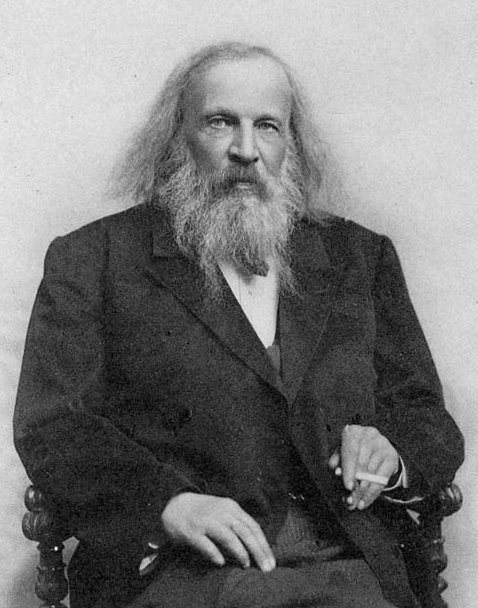
\includegraphics[width=\linewidth]{images/book1/mendeleev.jpg}

{\small Dmitri Mendelejev (1834--1907).}
\end{minipage}\hfill
\begin{minipage}[b]{0.6\linewidth}\centering
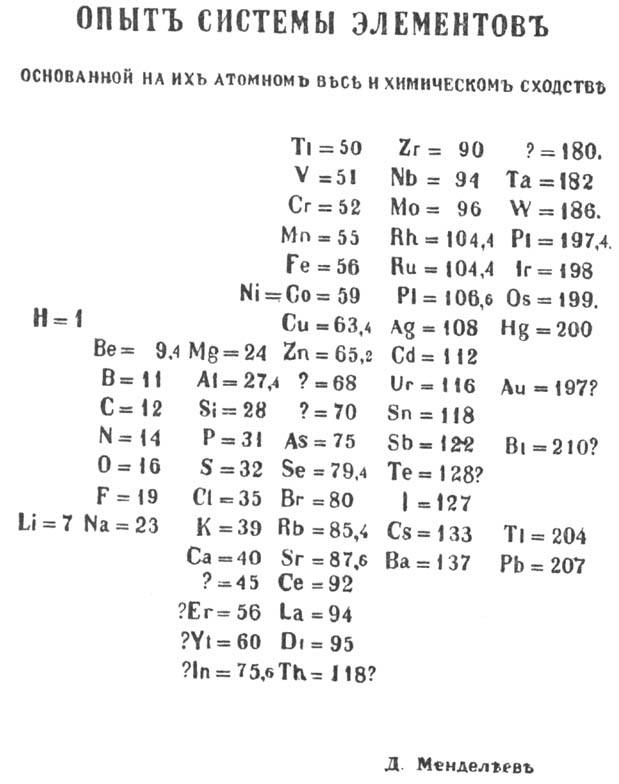
\includegraphics[width=0.85\linewidth]{images/book1/mendeleev-1869.jpg}

{\small De tabel van Mendelejev uit 1869, in het Russisch. Naast Si $= 28$
en Al $= 27.4$ wachten de gaten ``? $= 70$'' en ``? $= 68$'' op germanium
en gallium.}
\end{minipage}
\end{omfigure}

\begin{remark}[Volgorde naar atoomnummer]\label{rem:g9:periodic-table-first-look:order}
Mendelejev ordende de elementen naar atoomgewicht, en moest een paar
paren omwisselen, zoals telluur en jood, om de families bij elkaar te
houden. Tegenwoordig is de tabel geordend naar \omterm{def:g9:inside-the-atom:atomic-number}{atoomnummer}, dat pas later
ontdekt werd, en zijn die omwisselingen niet meer nodig.
\end{remark}

\section{Oefeningen}

\begin{exercise}[$\star$]\label{exo:g9:periodic-table-first-look:1}
In welke volgorde staan de elementen in het \omterm{def:g9:periodic-table-first-look:periodic-table}{periodiek systeem}?
\end{exercise}

\begin{exercise}[$\star$]\label{exo:g9:periodic-table-first-look:2}
Geef de \omterm{def:g9:periodic-table-first-look:period}{periode} en de groep van: koolstof ($Z = 6$), magnesium
($Z = 12$), argon ($Z = 18$).
\end{exercise}

\begin{exercise}[$\star$]\label{exo:g9:periodic-table-first-look:3}
\omterm{def:g9:periodic-table-first-look:metal}{Metaal} of \omterm{def:g9:periodic-table-first-look:metal}{niet-metaal}: ijzer, zwavel, koper, zuurstof, aluminium,
chloor?
\end{exercise}

\begin{exercise}[$\star$]\label{exo:g9:periodic-table-first-look:4}
Welk element staat in de tabel direct onder natrium? En direct onder
chloor?
\end{exercise}

\begin{exercise}[$\star\star$]\label{exo:g9:periodic-table-first-look:5}
Geef met de tabel de naam van het element in \omterm{def:g9:periodic-table-first-look:period}{periode} 4 en \omterm{def:g9:periodic-table-first-look:period}{groep} 2, en
van het element in \omterm{def:g9:periodic-table-first-look:period}{periode} 2 en \omterm{def:g9:periodic-table-first-look:period}{groep} 15.
\end{exercise}

\begin{exercise}[$\star\star$]\label{exo:g9:periodic-table-first-look:6}
Waarom kun je verwachten dat kalium, net als natrium, met water
reageert?
\end{exercise}

\begin{exercise}[$\star\star$]\label{exo:g9:periodic-table-first-look:7}
Een glanzend element geleidt elektrische stroom en vormt het \omterm{def:g9:ions:ion}{ion}
\ce{X^{2+}}. Is het een \omterm{def:g9:periodic-table-first-look:metal}{metaal} of een \omterm{def:g9:periodic-table-first-look:metal}{niet-metaal}? Leg uit.
\end{exercise}

\begin{exercise}[$\star\star$]\label{exo:g9:periodic-table-first-look:8}
Waarom liet Mendelejev gaten open in zijn tabel? Waarom was dat een
sterk punt van zijn tabel en geen zwakte?
\end{exercise}

\begin{exercise}[$\star\star$]\label{exo:g9:periodic-table-first-look:9}
Kijk naar de tabel van Mendelejev uit 1869. Welke atoomgewichten gaf hij
voor koolstof en voor zuurstof? Welke twee gaten, met een vraagteken
aangegeven, staan naast aluminium en silicium?
\end{exercise}

\begin{exercise}[$\star\star$]\label{exo:g9:periodic-table-first-look:10}
Hoeveel elementen zijn er in \omterm{def:g9:periodic-table-first-look:period}{periode} 2? En in \omterm{def:g9:periodic-table-first-look:period}{periode} 4?
\end{exercise}

\begin{exercise}[$\star\star\star$]\label{exo:g9:periodic-table-first-look:11}
Helium, neon en argon reageren met bijna niets. In welke groep staan
ze? Waarvoor zou je ze, gezien die eigenschap, kunnen gebruiken?
\end{exercise}

\begin{exercise}[$\star\star\star$]\label{exo:g9:periodic-table-first-look:12}
Gallium, onder aluminium, werd in 1875 ontdekt. Mendelejev had er een
atoomgewicht voor voorspeld dat dicht bij het gemiddelde lag van zijn
buren aluminium (27.0) en indium (114.8). Bereken dat gemiddelde.
(Gallium: 69.7.)
\end{exercise}

\section{Probleem: Het gat van Mendelejev}

\begin{problem}[{Weekendprobleem --- het atoomgewicht van een ontbrekend
element voorspellen uit zijn vier buren}]
\label{pb:g9:periodic-table-first-look:1}
% ledger: aw:Si, aw:Sn, aw:Ga, aw:As, aw:Ge, mend:eka-si-aw, ge:winkler-aw
In 1871 voorspelde Mendelejev de eigenschappen van eka-silicium, het
element dat onder silicium ontbrak. Een van zijn ideeën was dat de
eigenschappen van een element liggen tussen die van zijn buren erboven en
eronder, links en rechts. De huidige atoomgewichten van de vier buren van
het gat zijn: silicium 28.1 (erboven), tin 118.7 (eronder), gallium 69.7
(links), arseen 74.9 (rechts).

\medskip
\noindent\textbf{Deel I --- Het gat.}
\begin{enumerate}
  \item Zoek met het \omterm{def:g9:periodic-table-first-look:periodic-table}{periodiek systeem} van dit hoofdstuk het
        \omterm{def:g9:inside-the-atom:atomic-number}{atoomnummer}, de \omterm{def:g9:periodic-table-first-look:period}{periode} en de groep van germanium op, het element
        dat het gat opvult.
  \item Welk element staat erboven, welk eronder, welk links, welk
        rechts?
  \item Is germanium een \omterm{def:g9:periodic-table-first-look:metal}{metaal}, een \omterm{def:g9:periodic-table-first-look:metal}{niet-metaal} of een metalloïde?
  \item Waarom verwachtte Mendelejev dat het ontbrekende element op
        silicium zou lijken?
\end{enumerate}

\medskip
\noindent\textbf{Deel II --- Gemiddelden.}
\begin{enumerate}[resume]
  \item Bereken het gemiddelde van de atoomgewichten van de elementen
        boven en onder het gat.
  \item Bereken het gemiddelde van de atoomgewichten van de elementen
        links en rechts.
  \item Welk van de twee gemiddelden ligt dichter bij het echte
        atoomgewicht van germanium, 72.6? Waardoor zou dat kunnen komen?
  \item In zijn tabel van 1869 had Mendelejev voor dit gat ``? $= 70$''
        geschreven. Hoeveel zat hij ernaast?
\end{enumerate}

\medskip
\noindent\textbf{Deel III --- De voorspelling.}
\begin{enumerate}[resume]
  \item Bereken het gemiddelde van alle vier de buren, op één decimaal.
  \item In 1871 voorspelde Mendelejev 72; in 1886 mat Winkler 72.3.
        Vergelijk met jouw gemiddelde.
  \item Waarom overtuigde de ontdekking van germanium veel scheikundigen
        ervan dat de tabel van Mendelejev klopte?
  \item Geef je voorspelling: het atoomgewicht van eka-silicium uit het
        gemiddelde van zijn vier buren.
\end{enumerate}
\end{problem}
